\documentclass[aspectratio=169,11pt]{beamer}
\usetheme{default}
\setbeamertemplate{navigation symbols}{}
\setbeamertemplate{footline}{%
  \hfill\insertframenumber/\inserttotalframenumber\hspace*{4pt}\vspace{2pt}%
}
\usepackage{lmodern}
\usepackage[most]{tcolorbox}
\usepackage{listings}
\usepackage{tikz}
\usetikzlibrary{arrows.meta,positioning,shapes.geometric,fit,backgrounds}
\usepackage{booktabs}
\usepackage{hyperref}

\definecolor{lcgreen}{HTML}{2E7D32}
\definecolor{lcblue}{HTML}{1565C0}
\definecolor{lcorange}{HTML}{EF6C00}
\definecolor{lcred}{HTML}{C62828}
\definecolor{codebg}{HTML}{F5F5F5}
\definecolor{docgray}{gray}{0.55}

\newtcolorbox{conceptbox}[1][]{colback=yellow!20,colframe=yellow!60!black,title=#1,fonttitle=\bfseries,top=2pt,bottom=2pt,left=4pt,right=4pt}
\newtcolorbox{warningbox}[1][]{colback=red!15,colframe=red!60!black,title=#1,fonttitle=\bfseries,top=2pt,bottom=2pt,left=4pt,right=4pt}
\newtcolorbox{tipbox}[1][]{colback=green!10,colframe=green!50!black,title=#1,fonttitle=\bfseries,top=2pt,bottom=2pt,left=4pt,right=4pt}
\newtcolorbox{codebox}[1][]{colback=blue!10,colframe=blue!40!black,title=#1,fonttitle=\bfseries,top=2pt,bottom=2pt,left=4pt,right=4pt}

\lstset{
  basicstyle=\ttfamily\scriptsize,
  backgroundcolor=\color{codebg},
  breaklines=true,
  frame=single,
  rulecolor=\color{blue!40!black},
  keywordstyle=\color{lcblue}\bfseries,
  stringstyle=\color{lcgreen},
  commentstyle=\color{docgray}\itshape,
  language=Python,
  showstringspaces=false,
  tabsize=2,
  xleftmargin=2pt,
  xrightmargin=2pt,
  aboveskip=2pt,
  belowskip=2pt,
}

\newcommand{\docref}[1]{{\scriptsize\color{docgray}[Docs: #1]}}

\title{Section 04: Tool Integration}
\subtitle{Giving Graphs the Ability to Interact with the World}
\author{LangGraph v1.0.x (March 2026)}
\date{}

\begin{document}

\frame{\titlepage}

\begin{frame}{Mental Model: Tool Integration}
  \begin{conceptbox}[The Big Picture]
    \setlength{\itemsep}{1pt}
    \begin{itemize}
      \item Tools let graphs \textbf{act on the world}: execute code, query databases, call APIs
      \item Model generates \textbf{tool calls}, ToolNode \textbf{executes} them, results flow back
      \item Creates a \textbf{feedback loop}: observe -> reason → act → observe
      \item Foundation for agents, task automation, and agentic behavior
    \end{itemize}
  \end{conceptbox}
  \vspace{0.1cm}
  \begin{tipbox}[Why This Matters]
    Without tools, LLMs are isolated. Tools unlock real-world impact.
  \end{tipbox}
\end{frame}

\begin{frame}{What Are Tools in LangGraph?}
  \begin{conceptbox}[Tool Definition]
    \setlength{\itemsep}{1pt}
    \begin{itemize}
      \item Callable functions that an LLM can \textbf{request} (not execute directly)
      \item Have a \textbf{schema}: name, description, input spec, return type
      \item Bound to models so they know tools exist: \texttt{model.bind\_tools()}
      \item Executed by \textbf{ToolNode}, not by the model itself
    \end{itemize}
  \end{conceptbox}
  \vspace{0.1cm}
  \begin{codebox}[Tool Ecosystem]
    \setlength{\itemsep}{1pt}
    \begin{itemize}
      \item \texttt{@tool} decorator: simple functions
      \item \texttt{StructuredTool}: complex schemas with Pydantic
      \item \texttt{ToolNode}: prebuilt executor
      \item \texttt{tools\_condition}: prebuilt router
    \end{itemize}
  \end{codebox}
\end{frame}

\begin{frame}[fragile]{Defining Tools with @tool Decorator}
  \begin{codebox}[Basic Tool Definition]
    \begin{lstlisting}
from langchain_core.tools import tool
@tool
def get_weather(location: str) -> str:
  """Get current temperature in location."""
  return f"Weather in {location}: 72°F"
@tool
def add_numbers(a: int, b: int) -> int:
  """Add two numbers."""
  return a + b
    \end{lstlisting}
  \end{codebox}
  \vspace{0.1cm}
  \begin{tipbox}[Key Points]
    \setlength{\itemsep}{1pt}
    \begin{itemize}
      \item Docstring becomes the tool \textbf{description}
      \item Type hints drive schema inference
      \item Minimal boilerplate, quick prototyping
    \end{itemize}
  \end{tipbox}
\end{frame}

\begin{frame}[fragile]{StructuredTool for Complex Schemas}
  \begin{codebox}[Pydantic Schema]
    \begin{lstlisting}
from pydantic import BaseModel, Field
from langchain_core.tools import StructuredTool
class QueryInput(BaseModel):
  query: str = Field(..., description="Search term")
  limit: int = Field(default=10, description="Max results")
def search_docs(query: str, limit: int) -> str:
  return f"Search: {query}, Limit: {limit}"
tool = StructuredTool.from_function(
  func=search_docs,
  args_schema=QueryInput
)
    \end{lstlisting}
  \end{codebox}
  \vspace{0.1cm}
  \begin{conceptbox}[When to Use]
    StructuredTool when your tool needs complex validation, optional params, or detailed field descriptions.
  \end{conceptbox}
\end{frame}

\begin{frame}[fragile]{Binding Tools to Chat Models}
  \begin{codebox}[model.bind\_tools()]
    \begin{lstlisting}
from langchain_openai import ChatOpenAI
model = ChatOpenAI(model="gpt-4")
tools = [get_weather, add_numbers]
bound_model = model.bind_tools(tools)
response = bound_model.invoke(
  "What's the weather in NYC?"
)
print(response.tool_calls)
    \end{lstlisting}
  \end{codebox}
  \vspace{0.1cm}
  \begin{tipbox}[What Binding Does]
    \setlength{\itemsep}{1pt}
    \begin{itemize}
      \item Sends tool schemas to model in API call
      \item Model learns what tools are available
      \item Model can decide to call tools via \texttt{tool\_calls}
    \end{itemize}
  \end{tipbox}
\end{frame}

\begin{frame}[fragile,shrink=15]{ToolNode: The Prebuilt Executor}
  \begin{codebox}[Using ToolNode]
    \begin{lstlisting}
from langgraph.prebuilt import ToolNode
tool_node = ToolNode(tools=[get_weather, add_numbers])
state = {
  "messages": [
    HumanMessage("What's the weather in NYC?"),
    AIMessage(
      content="",
      tool_calls=[{
        "id": "call_1",
        "name": "get_weather",
        "args": {"location": "NYC"}
      }]
    )
  ]
}
result = tool_node.invoke(state)
    \end{lstlisting}
  \end{codebox}
  \vspace{0.1cm}
  \begin{tipbox}[What ToolNode Does]
    \setlength{\itemsep}{1pt}
    \begin{itemize}
      \item Executes \texttt{tool\_calls} from model messages
      \item Returns \texttt{ToolMessage} results back to state
    \end{itemize}
  \end{tipbox}
\end{frame}

\begin{frame}{Tool-Calling Loop: How It Works}
  \begin{conceptbox}[The Flow]
    \setlength{\itemsep}{1pt}
    \begin{itemize}
      \item \textbf{1. User query} arrives at graph
      \item \textbf{2. Model} (with bound tools) processes message
      \item \textbf{3. Model generates} \texttt{tool\_calls} if needed
      \item \textbf{4. ToolNode} executes the calls
      \item \textbf{5. ToolMessages} with results added to state
      \item \textbf{6. Model} processes results and responds
      \item \textbf{Loop} repeats until model stops calling tools
    \end{itemize}
  \end{conceptbox}
\end{frame}

\begin{frame}{TikZ Diagram: The Tool-Calling Loop}
  \begin{center}
    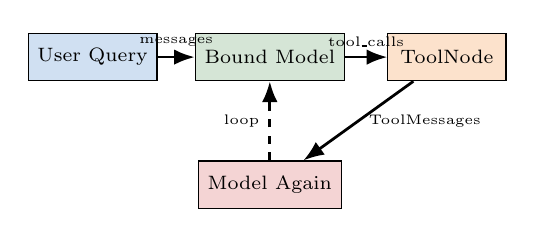
\begin{tikzpicture}[scale=0.9, every node/.style={font=\scriptsize}]
      \node[draw, rectangle, fill=lcblue!20, minimum width=1.5cm, minimum height=0.6cm] (user) at (0, 2) {User Query};
      \node[draw, rectangle, fill=lcgreen!20, minimum width=1.5cm, minimum height=0.6cm] (model) at (2.5, 2) {Bound Model};
      \node[draw, rectangle, fill=lcorange!20, minimum width=1.5cm, minimum height=0.6cm] (toolnode) at (5, 2) {ToolNode};
      \node[draw, rectangle, fill=lcred!20, minimum width=1.5cm, minimum height=0.6cm] (result) at (2.5, 0.2) {Model Again};
      \draw[-Latex, line width=1pt] (user) -- (model) node[midway, above] {\tiny messages};
      \draw[-Latex, line width=1pt] (model) -- (toolnode) node[midway, above] {\tiny tool\_calls};
      \draw[-Latex, line width=1pt] (toolnode) -- (result) node[midway, right] {\tiny ToolMessages};
      \draw[-Latex, line width=1pt, dashed] (result) -- (model) node[midway, left] {\tiny loop};
    \end{tikzpicture}
  \end{center}
  \vspace{0.1cm}
  \begin{tipbox}[Key Insight]
    Model never executes tools; it only \textbf{requests} them. ToolNode handles execution.
  \end{tipbox}
\end{frame}

\begin{frame}[fragile]{Building a Complete Tool-Calling Graph}
  \begin{codebox}[Step-by-Step Graph]
    \begin{lstlisting}
from langgraph.graph import StateGraph, START, END
from langgraph.prebuilt import ToolNode, tools_condition
builder = StateGraph(MessagesState)
builder.add_node("model", model_node)
builder.add_node("tools", ToolNode(tools=[...]))
builder.add_edge(START, "model")
builder.add_conditional_edges(
  "model", tools_condition,
  {"tools": "tools", END: END}
)
builder.add_edge("tools", "model")
graph = builder.compile()
    \end{lstlisting}
  \end{codebox}
\end{frame}

\begin{frame}[fragile]{tools\_condition: The Prebuilt Router}
  \begin{codebox}[What tools\_condition Does]
    \begin{lstlisting}
from langgraph.prebuilt import tools_condition
def decide_next(state) -> str:
  if state["messages"][-1].tool_calls:
    return "tools"
  else:
    return END
builder.add_conditional_edges(
  "model", tools_condition,
  {"tools": "tools", END: END}
)
    \end{lstlisting}
  \end{codebox}
  \vspace{0.1cm}
  \begin{tipbox}[Why Use tools\_condition]
    Eliminates boilerplate: it already knows how to route based on tool calls.
  \end{tipbox}
\end{frame}

\begin{frame}{Handling Tool Errors Gracefully}
  \begin{warningbox}[Common Error Scenarios]
    \setlength{\itemsep}{1pt}
    \begin{itemize}
      \item Tool function raises exception
      \item Model calls nonexistent tool (schema mismatch)
      \item Tool returns invalid data type
    \end{itemize}
  \end{warningbox}
  \vspace{0.1cm}
  \begin{conceptbox}[Best Practices]
    \setlength{\itemsep}{1pt}
    \begin{itemize}
      \item Wrap tool calls in try-catch
      \item Return error messages as ToolMessages
      \item Let model retry with context
    \end{itemize}
  \end{conceptbox}
\end{frame}

\begin{frame}[fragile]{Handling Tool Errors: Example}
  \begin{codebox}[Error Handling Pattern]
    \begin{lstlisting}
def safe_tool_call(tool_name, args):
  try:
    func = tools_dict[tool_name]
    return func(**args)
  except Exception as e:
    return f"Error: {str(e)}"
def tool_node_with_errors(state):
  for call in state["messages"][-1].tool_calls:
    result = safe_tool_call(
      call["name"], call["args"]
    )
    state["messages"].append(
      ToolMessage(result, tool_call_id=call["id"])
    )
  return state
    \end{lstlisting}
  \end{codebox}
\end{frame}

\begin{frame}{Multiple Tools: Registration and Routing}
  \begin{conceptbox}[Multi-Tool Patterns]
    \setlength{\itemsep}{1pt}
    \begin{itemize}
      \item Register all tools: \texttt{model.bind\_tools([tool1, tool2, ...])}
      \item ToolNode automatically routes by tool name
      \item Model learns all schemas and picks best tool
      \item Add tools dynamically at graph creation time
    \end{itemize}
  \end{conceptbox}
  \vspace{0.1cm}
  \begin{tipbox}[Tool Naming]
    Use clear, unique names. Model picks tools by matching names to \texttt{tool\_calls}.
  \end{tipbox}
\end{frame}

\begin{frame}[fragile]{Tool Call Validation and Sanitization}
  \begin{codebox}[Validation Example]
    \begin{lstlisting}
from pydantic import validator
class SearchInput(BaseModel):
  query: str = Field(..., min_length=1)
  limit: int = Field(default=10, ge=1, le=100)
  @validator('query')
  def query_not_sql(cls, v):
    if 'DROP' in v.upper():
      raise ValueError("SQL injection attempt")
    return v
    \end{lstlisting}
  \end{codebox}
  \vspace{0.1cm}
  \begin{warningbox}[Always Validate]
    Never trust model-generated tool args. Use Pydantic validators for safety.
  \end{warningbox}
\end{frame}

\begin{frame}[fragile]{Async Tool Execution}
  \begin{codebox}[Async Tools]
    \begin{lstlisting}
import asyncio
@tool
async def fetch_data_async(url: str) -> str:
  """Async fetch from URL."""
  # In real code, use aiohttp
  await asyncio.sleep(0.1)
  return f"Data from {url}"
async def run_graph():
  result = await graph.ainvoke(
    input={"messages": [...]},
    config={...}
  )
    \end{lstlisting}
  \end{codebox}
  \vspace{0.1cm}
  \begin{tipbox}[Performance Boost]
    Use async tools for I/O-bound operations (API calls, DB queries).
  \end{tipbox}
\end{frame}

\begin{frame}[fragile]{Custom Tool Nodes}
  \begin{codebox}[When ToolNode Isn't Enough]
    \begin{lstlisting}
def custom_tool_node(state):
  """Add logging, custom routing, etc."""
  for call in state["messages"][-1].tool_calls:
    print(f"Executing: {call['name']}")
    result = execute_tool(call["name"], call["args"])
    state["messages"].append(
      ToolMessage(result, tool_call_id=call["id"])
    )
  return state
builder.add_node("custom_tools", custom_tool_node)
    \end{lstlisting}
  \end{codebox}
  \vspace{0.1cm}
  \begin{tipbox}[Use Cases]
    Logging, rate limiting, custom error handling, tool chaining.
  \end{tipbox}
\end{frame}

\begin{frame}{Common Pitfalls}
  \begin{warningbox}[Tool Schema Mismatch]
    \setlength{\itemsep}{1pt}
    \begin{itemize}
      \item Model calls tool with wrong argument names
      \item Solution: verify Pydantic schema matches function signature
    \end{itemize}
  \end{warningbox}
  \vspace{0.1cm}
  \begin{warningbox}[Forgetting to Bind Tools]
    \setlength{\itemsep}{1pt}
    \begin{itemize}
      \item Model has no knowledge of tools if not bound
      \item Solution: always call \texttt{model.bind\_tools()} before graph
    \end{itemize}
  \end{warningbox}
  \vspace{0.1cm}
  \begin{warningbox}[Misplaced ToolNode]
    \setlength{\itemsep}{1pt}
    \begin{itemize}
      \item ToolNode must come \textbf{after} model in graph
      \item Solution: use \texttt{tools\_condition} for proper routing
    \end{itemize}
  \end{warningbox}
\end{frame}

\begin{frame}[fragile]{Summary: Tool Integration Cheat Sheet}
  \begin{codebox}[Quick Reference]
    \begin{lstlisting}
@tool
def my_tool(x: int) -> int:
  """Tool docstring."""
  return x * 2
model = ChatOpenAI(...).bind_tools([my_tool])
from langgraph.prebuilt import ToolNode, tools_condition
tool_node = ToolNode([my_tool])
builder.add_conditional_edges(
  "model", tools_condition,
  {"tools": "tools", END: END}
)
    \end{lstlisting}
  \end{codebox}
\end{frame}

\begin{frame}{Self-Check: Do You Understand?}
  \begin{enumerate}
    \setlength{\itemsep}{1pt}
    \item How does \texttt{bind\_tools()} change what a model can do?
    \item What's the difference between \texttt{@tool} and \texttt{StructuredTool}?
    \item Why doesn't the model execute tools directly?
    \item How does \texttt{tools\_condition} avoid boilerplate?
    \item What happens if a tool raises an exception?
    \item When should you create a custom tool node?
    \item How do you handle multiple tools in one graph?
  \end{enumerate}
\end{frame}

\end{document}
